\subsection{Manipulator on a fixed spherical base}
An R\&D project was presented in \cite{motta2010prototype} to propose
methodology, simulation and the steps for building a robotic system to repair
hydraulic turbine blades, % The robotic system does repair using the arc welding
%technology before held manually 
 in highly dangerous environments with $ 40^o C$ to $ 99^o C$, and 10 operation
 hours.
%Um projeto de pesquisa e desenvolvimento foi apresentado em
%\cite{motta2010prototype} com o objetivo de propor metodologia, simulação e
%os passos para construção de um sistema robótico para recuperar danos materiais
%em pás de turbinas hidráulicas. O sistema robótico faz
%reparo utilizando a tecnologia de soldagem a arco elétrico, antes realizada
%manualmente em ambientes de alta periculosidade com temperaturas que variam
%entre $40^o C$ e $99^o C$, e operações que duram em torno de 10 horas. 

The robot meets the following requirements: ability to operate in any position:
horizontal, vertical, reversed; lightweight for portability and blade fixation;
stiffness to deflection: payload on the wrist occurs in any direction and
extension; high precision; parts availability on the market; user interface;
large workspace; adhesion to the hydraulic turbine blades.

%O robô deve atender aos seguintes requisitos:
%\begin{itemize}
%  \item Capacidade de operar em qualquer posição: horizontal, vertical,
%  invertida;
%  \item Pouco peso para portabilidade e fixação às pás;
%  \item Rigidez à deflexão: carga no punho do manipulador ocorre em qualquer
%  direção e extensão;
%  \item Grande precisão;
%  \item Disponibilidade de peças no mercado;
%  \item Controle com interface de usuário;
%  \item Grande área de trabalho;
%  \item Facilidade de adesão às pás de turbinas hidráulicas.
%\end{itemize}

The system has spherical topology and the following characteristics: manipulator
with three DOF (2R1P) and wrist with two DOF (2R); 3D surface mapping with laser
scanner; embedded electronics; arc welding gun; blade adhesion by magnetic or
suction devices; low cost; ring-shaped workspace with 2.5 m, and 60 cm height;
30 kg weight and dimensions 30 x 25 x 100 cm; and autonomy.
%A solução para o sistema robótico apresenta topologia esférica, como pode ser
%visto na figura~\ref{fig:esferico} e características:

%\begin{figure}[ht]
%\centering
%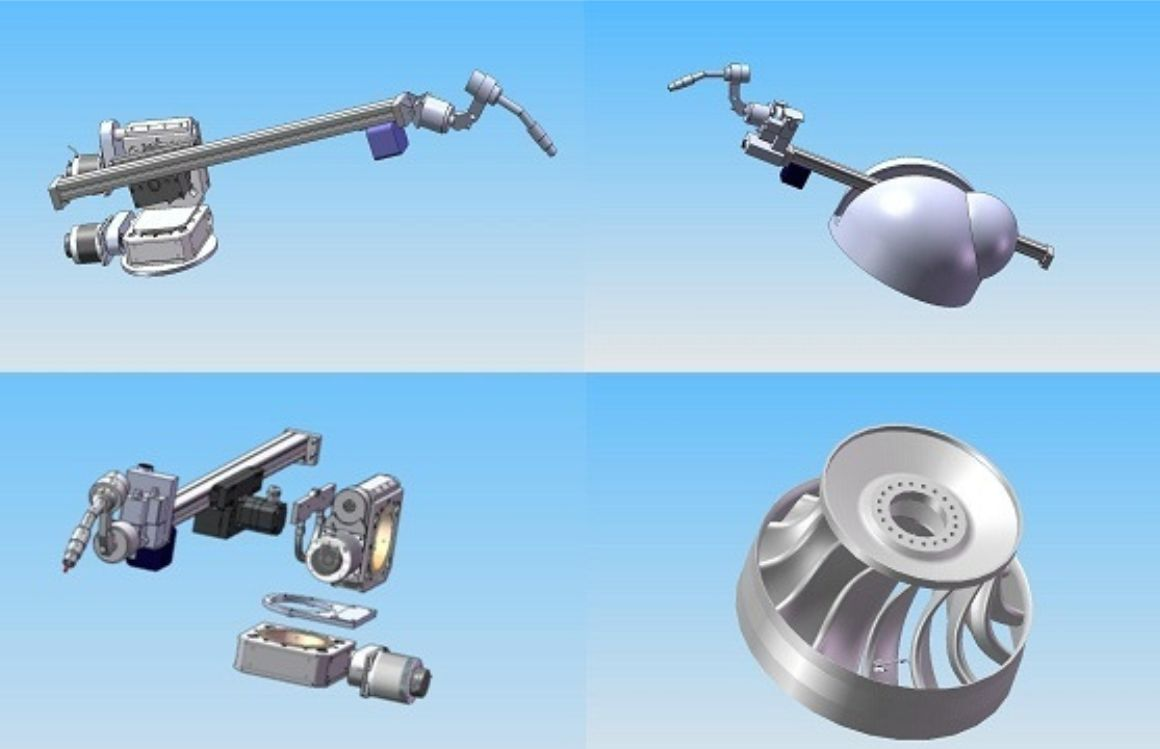
\includegraphics[width=8.4cm]{figs/esferico/esferico.jpg}
%\caption{Illustration of the robotic system with spherical base}
%\label{fig:esferico}
%\end{figure}

%\begin{itemize}
%   \item manipulator with three DOF (2R1P) and wrist with two DOF (2R);
%   \item 3D surface mapping with laser scanner;
%   \item embedded electronics;
%   \item arc welding;
%   \item blade adhesion by magnetic or suction devices;
%   \item low cost;
%   \item ring-shaped workspace with 2.5 m, and 60 cm height;
%   \item 30 kg weight and dimensions 30 x 25 x 100 cm;
%   \item autonomous manipulator;
%\end{itemize}

%\begin{itemize}
%  \item Três (3) graus de liberdade no manipulador (2R1P) e dois graus de
%  liberdade no punho (2R);
%  \item Mapeamento de superfície 3D com laser;
%  \item Eletrônica embarcada;
%  \item Soldagem por arco elétrico;
%  \item Fixação nas pás por dispositivos magnéticos ou de sucção;
%  \item Baixo custo;
%  \item Área de trabalho em forma de anel com 2.5 m e 60 cm de altura;
%  \item Peso 30 kg e dimensões 30 x 25 x 100 cm;
%  \item Robô com manipulador autônomo;
%\end{itemize}

The robotic manipulator system with spherical base is a compatible solution
for the HVOF application in hydraulic turbine blades, since its
original application is blade repair by arc welding, same environment and
similar challenge. All the system advantages and features are applicable to
the solution of a HVOF system. However, there are particular challenges in the
HVOF process, which are disadvantages of the solution: the HVOF must be
performed in the entire blade, thus the positions of the system must be
manually changed at least 2 times per blade side, and must be moved blade to
blade; the end effector must process the blade with great speed, as required
by the HVOF; complex adhesion system is also needed because blade temperature
range.

%O sistema robótico de manipulador com base esférica apresenta solução
% compatível para a aplicação de HVOF em pás de turbinas hidráulicas, já que sua aplicação
%original é soldagem das pás, semelhante ao desafio deste artigo. Todas as suas
%características são vantagens e aplicam-se à solução de um sistema para HVOF.
%Há, porém, desafios particulares na metalização das pás e que são desvantagens
%da solução:


%\textbf{Disadvantages:}
%\begin{itemize}
%   \item The HVOF must be performed in the entire blade. Therefore, the
%   positions of the system must be manually changed at least 2 times per blade
%   side, and must be moved blade to blade;
%   \item The end effector must process the blade with great speed, as
%   required by the HVOF.
%\end{itemize}

%\textbf{Desvantagens:}
%\begin{itemize}
%  \item A metalização deve ser realizada em toda a pá. Portanto, o sistema
%  deverá ser manualmente trocado de posição, pelo menos 4 vezes (duas posições
%  para a frente e duas posições para a região de trás). E deve ser trocado de
  % pá em pá;
%  \item O efetuador deve percorrer a pá com grande velocidade, como exige o
%  processo de metalização.
%\end{itemize}